\begin{table}[h]
  \centering
  \begin{tabular}{r|r|r}
    \textbf{N} & \textbf{build\_ns(rec)} & \textbf{build\_ns(iter)} \\ \hline
      1024   &         39\,342  &         33\,367  \\
      2048   &        127\,588  &        101\,058  \\
      4096   &        309\,710  &        254\,312  \\
      8192   &        815\,879  &        644\,740  \\
     16384   &     2\,116\,781  &     1\,641\,328  \\
     32768   &     4\,968\,198  &     3\,924\,036  \\
     65535   &    13\,675\,533  &     9\,617\,724  \\
    131072   &    32\,381\,978  &    23\,861\,046  \\

  \end{tabular}
  \caption{Build times (nanoseconds) for recursive vs iterative insert.}
  \label{tab:build-benchmark}
\end{table}


\begin{figure}[h]
  \centering
  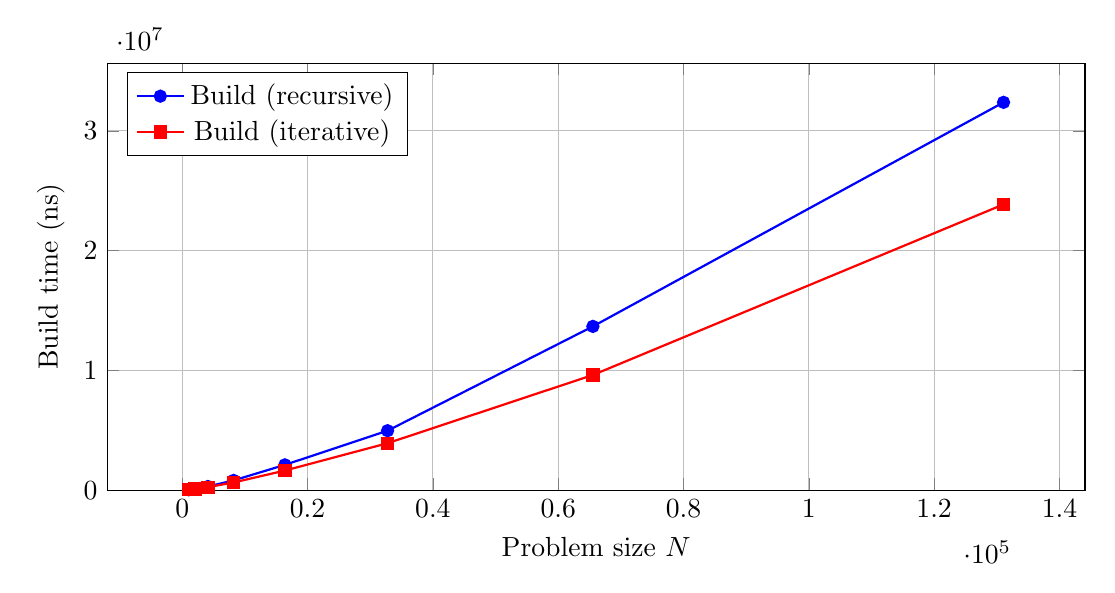
\begin{tikzpicture}
    \begin{axis}[
      xlabel={Problem size $N$},
      ylabel={Build time (ns)},
      width=14cm, height=7cm,
      grid=major,
      legend style={at={(0.02,0.98)}, anchor=north west, draw=black, fill=white},
      xmajorgrids=true, ymajorgrids=true,
      ymin=0
    ]

      \addplot[color=blue, mark=*, thick] coordinates {
        (1024, 39342)
        (2048, 127588)
        (4096, 309710)
        (8192, 815879)
        (16384, 2116781)
        (32768, 4968198)
        (65535, 13675533)
        (131072, 32381978)

      };
      \addlegendentry{Build (recursive)}

      \addplot[color=red, mark=square*, thick] coordinates {
        (1024, 33367)
        (2048, 101058)
        (4096, 254312)
        (8192, 644740)
        (16384, 1641328)
        (32768, 3924036)
        (65535, 9617724)
        (131072, 23861046)

      };
      \addlegendentry{Build (iterative)}

    \end{axis}
  \end{tikzpicture}
  \caption{Build benchmark: recursive vs iterative insertion across increasing $N$.}
  \label{fig:build-benchmark}
\end{figure}


\begin{table}[h]
  \centering
  \begin{tabular}{r|r|r}
    \textbf{N} & \textbf{lookup\_ns(BST)} & \textbf{lookup\_ns(binsearch)} \\ \hline
      1024   &                  19  &                      37  \\
      2048   &                  26  &                      43  \\
      4096   &                  35  &                      47  \\
      8192   &                  41  &                      52  \\
     16384   &                  52  &                      58  \\
     32768   &                  61  &                      67  \\
     65535   &                  83  &                      74  \\
    131072   &                 104  &                      84  \\

  \end{tabular}
  \caption{Lookup times (ns) for BST and array binary search.}
  \label{tab:lookup-benchmark}
\end{table}


\begin{figure}[h]
  \centering
  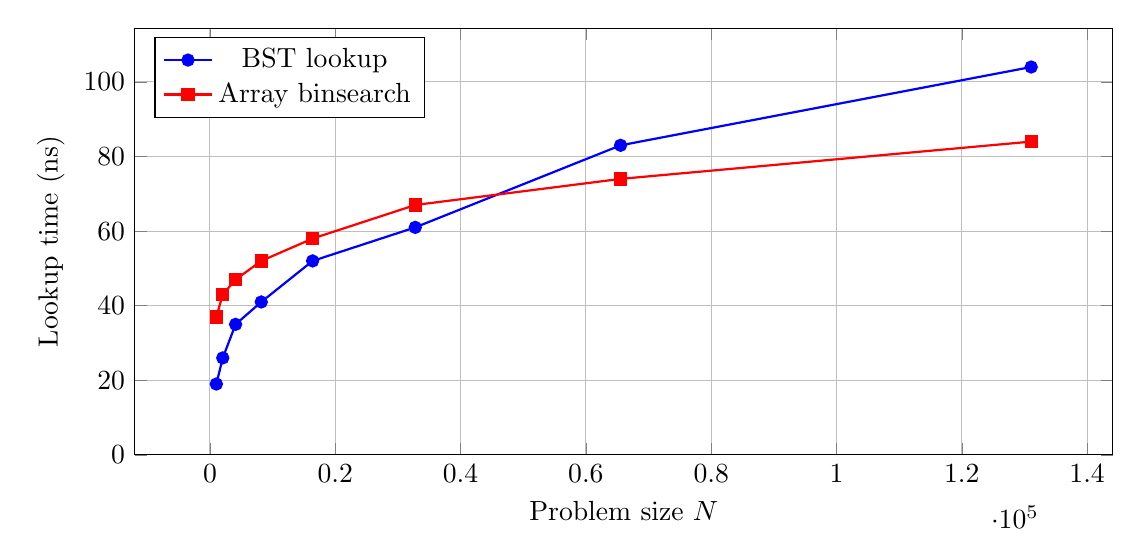
\begin{tikzpicture}
    \begin{axis}[
      xlabel={Problem size $N$},
      ylabel={Lookup time (ns)},
      width=14cm, height=7cm,
      grid=major,
      legend style={at={(0.02,0.98)}, anchor=north west, draw=black, fill=white},
      xmajorgrids=true, ymajorgrids=true,
      ymin=0
    ]

      \addplot[color=blue, mark=*, thick] coordinates {
        (1024, 19)
        (2048, 26)
        (4096, 35)
        (8192, 41)
        (16384, 52)
        (32768, 61)
        (65535, 83)
        (131072, 104)

      };
      \addlegendentry{BST lookup}

      \addplot[color=red, mark=square*, thick] coordinates {
        (1024, 37)
        (2048, 43)
        (4096, 47)
        (8192, 52)
        (16384, 58)
        (32768, 67)
        (65535, 74)
        (131072, 84)

      };
      \addlegendentry{Array binsearch}

    \end{axis}
  \end{tikzpicture}
  \caption{Lookup benchmark: BST vs array binary search.}
  \label{fig:lookup-benchmark}
\end{figure}

